\section{Die Arduino-Zukunft}

\begin{frame}
\frametitle{Quo Vadis, Arduino?}

Die Arduino-Familie f�cherte in den letzten Jahren immer mehr auf. Ein deutlicher Trend sind Platinen, die wie der Raspberry unter Linux laufen? Werden sie dem RPi gef�hrlich? Entfremdet sich Arduino von seiner urspr�nglichen Zielgruppe?

\end{frame}

\subsection{,,Starke'' Arduinos mit Linux}

\begin{frame}
\frametitle{Galileo}

Intel verschenkt an Unis Galileo-Boards im Arduino-Shield-Layout. Das besondere: Statt Microcontroller kommt ein Pentium zum Einsatz:

  \begin{center}
    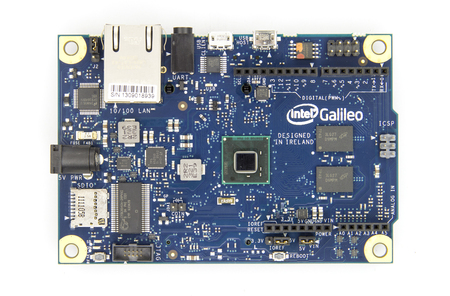
\includegraphics[width=8cm]{photos/galileo.jpg}
  \end{center}
\end{frame}

\begin{frame}
\frametitle{Galileo}

Intel verschenkt an Unis Galileo-Boards im Arduino-Shield-Layout. Das besondere: Statt Microcontroller kommt ein Pentium zum Einsatz:
\newline

\begin{itemize}
\item Intels Versuch, mit Embedded x86 in die N�he von Microcontrollern zu kommen
\item Referenzboard f�r Intels Quark SoC x1000
\item Arduino-Code wird in ELF-Objekte kompiliert
\item recht langsames IO
\item \emph{Mattias' Meinung:} The worst of both worlds
\end{itemize}
\end{frame}

\begin{frame}
\frametitle{Arduino Tre}
Gemeinsam mit TI und dem BeagleBone-Projekt entwickelter ,,janusk�pfiger'' Arduino aus TI Sitara und Atmega32u4, Leistung der Linux-Seite h�her als beim Raspberry Pi:

  \begin{center}
    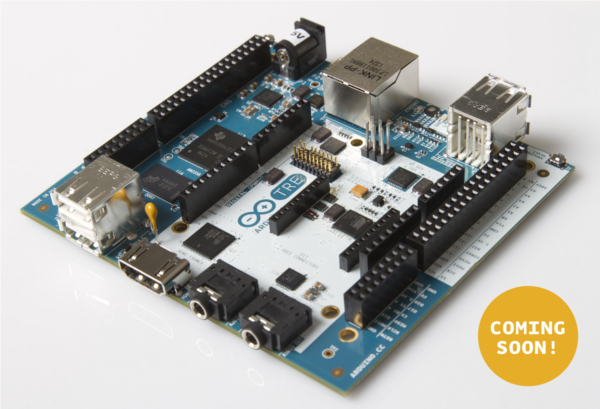
\includegraphics[width=8cm]{photos/arduinotre.jpg}
  \end{center}
\end{frame}

\begin{frame}
\frametitle{Arduino Tre}
Gemeinsam mit TI und dem BeagleBone-Projekt entwickelter ,,janusk�pfiger'' Arduino aus TI Sitara und Atmega32u4, Leistung der Linux-Seite h�her als beim Raspberry Pi:

\begin{itemize}
\item Von TI als Referenzplattform betrachtet
\item 100\% Code-Kompatibilit�t zu Arduino Leonardo
\item 100\% Code-Kompatibilit�t zu Beaglebone Black
\item recht teuer - Entwicklerkit 149 \euro - final 60 bis 80 \euro
\item \emph{Mattias' Meinung:} Tolles Konzept, hohe Leistung, aber hoher Preis und gro�e Platine
\end{itemize}
\end{frame}

\begin{frame}
\frametitle{Arduino Y�n}
Janusk�pfiger Arduino aus MIPS-Prozessor und Atmega32u4, Formfaktor des Uno, Leistung der Linux-Seite deutlich kleiner als beim Raspberry Pi, daf�r incl. WLAN und schnell angebundenem Ethernet:

  \begin{center}
    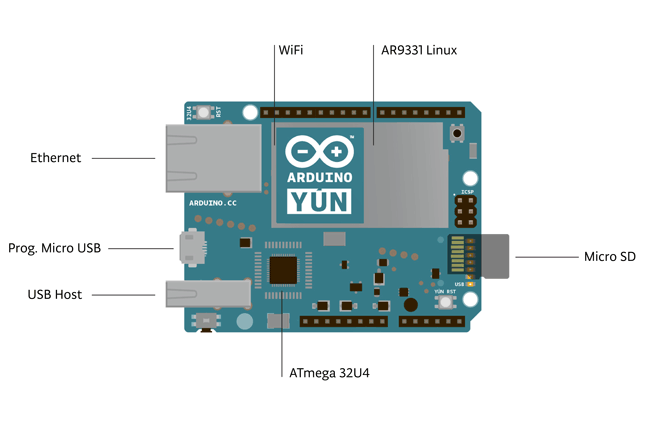
\includegraphics[width=8cm]{photos/YunParts.png}
  \end{center}
\end{frame}

\begin{frame}
\frametitle{Arduino Y�n}
Janusk�pfiger Arduino aus MIPS-Prozessor und Atmega32u4, Formfaktor des Uno, Leistung der Linux-Seite deutlich kleiner als beim Raspberry Pi, daf�r incl. WLAN und schnell angebundenem Ethernet:
\newline

\begin{itemize}
\item Eigenentwicklung mit Fokus auf guter Nutzbarkeit
\item 100\% Code-Kompatibilit�t zu Arduino Leonardo
\item OpenWRT basierte Distribution f�r die MIPS-Seite
\item Stra�enpreis 60 bis 75 \euro - kann parallel als WLAN Access Point genutzt werden
\item \emph{Mattias' Meinung:} Tolles Konzept, passende Leistung, sollte etwas g�nstiger sein
\item \emph{Der Clou:} Die Software - einfacher geht es nicht!
\end{itemize}
\end{frame}

\begin{frame}
\frametitle{Arduino Y�n - Software-Integration}
Eine neue Sammlung von Bibliotheken f�r die Arduino-IDE abstrahiert die Kommunikation zwischen Microcontroller- und Microprozessorseite:
\newline

\begin{itemize}
\item Bridge-Bibliothek f�r Zugriff auf viele Netzwerkfunktionen aus Arduino-Sketches - nur eine Programmiersprache n�tig!
\item ,,Mailbox'' (toter Briefkasten) f�r den Datenaustausch zwischen Microcontroller und Microprocessor
\item Integration von Temboo - abstrahiert verschiedene Webdienste
\item Voller Paketumfang von OpenWRT
\item Einfaches Webinterface f�r die Einrichtung - Luci bekannt von OpenWRT
\end{itemize}
\end{frame}

\begin{frame}
\frametitle{Arduino Y�n - Twitter-Beispiel}
  \begin{center}
    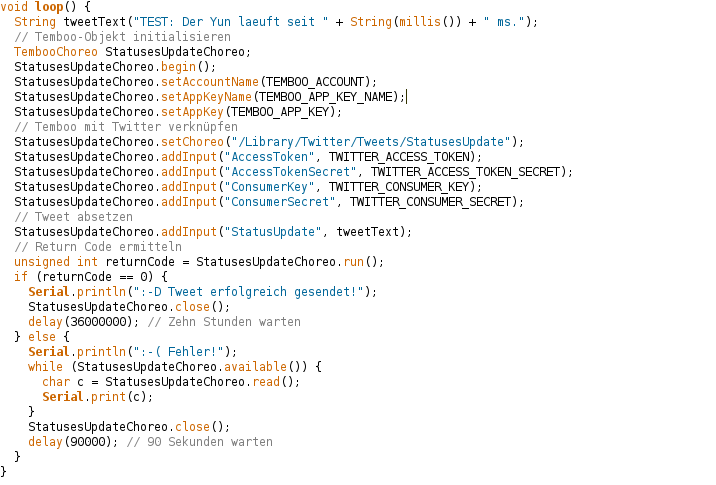
\includegraphics[width=10cm]{photos/codetwitter.png}
  \end{center}
\end{frame}

\begin{frame}
\frametitle{Arduino Y�n - Tweets ganz praktisch}
  \begin{center}
    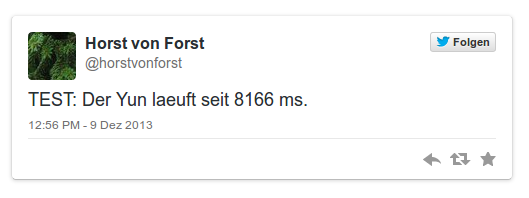
\includegraphics[width=9cm]{photos/tweet.png}
  \end{center}

Wozu? ,,Horst von Forst'', unser Weihnachtsbaum twitterte, wenn er zuwenig Wasser hatte. Der vollst�ndige Code und Erkl�rungen zum verwendeten Sensor unter: http://www.arduino-hausautomation.de/
\end{frame}

\subsection{Neue Microcontroller mit ARM-Kern}

\begin{frame}
\frametitle{Arduino Due}
Erstes Arduino-Board mit 32Bit-ARM-Microcontroller. Ca. 45 \euro. CAN-Interface. Blick in die Zukunft ohne weitere Relevanz. Daher keine technischen Details:

  \begin{center}
    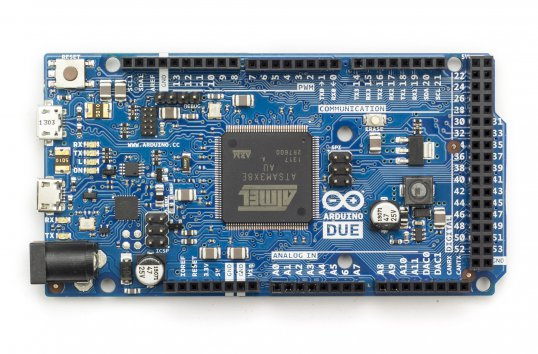
\includegraphics[width=8cm]{photos/arduinodue.jpg}
  \end{center}
\end{frame}

\begin{frame}
\frametitle{Arduino Zero}
Designierter Nachfolger des Arduino Uno mit SAMD21G18, h�here Integration verspricht g�nstigere Preise:

  \begin{center}
    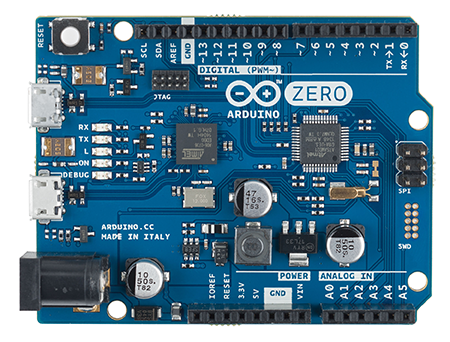
\includegraphics[width=8cm]{photos/arduinozero.png}
  \end{center}
\end{frame}

\begin{frame}
\frametitle{Arduino Zero}
Designierter Nachfolger des Arduino Uno mit SAMD21G1, h�here Integration verspricht g�nstigere Preise:
\newline 

\begin{itemize}
\item 32 Bit Microcontroller mit ARM-Kern
\item 256kB Flash 
\item 32kB SRAM 
\item Hohe Integration mit Debugger und 2xUSB
\item Tendenziell Preise auf Level von Atmega32u4 oder Atmega328P - kleine Klone f�r weniger als 5 \euro\  m�glich
\item \textbf{Achtung!} 3,3 Volt
\item \textbf{Achtung!} kein DIL Package des Controllers erh�ltlich
\end{itemize}

\end{frame}

\subsection{Problem Fragmentierung}

\begin{frame}
\frametitle{Bitte unterbrechen!}

\textbf{Falls Mattias in diesem Abschnitt ausschweift, bitte unterbrechen!}

\end{frame}


\begin{frame}
\frametitle{Microcontroller-Familien von Arduino}

Im Laufe der Jahre wurden von Arduino immer mehr Microcontroller-Familien unterst�tzt, nicht nur kleine Spr�nge wie von Atmega168 auf Atmega328, sondern mehrere Br�che. Offizielle Familien:
\newline

\begin{itemize} 
\item Atmega328: Arduino Uno, Pro Mini
\item Atmega32u4: Leonardo, Y�n, Micro
\item Atmega2560: Mega2560
\item \emph{neu} ATSAMD21: Arduino Zero, Due
\item \emph{neu} Intel Galileo - noch nicht eingepflegt in Arduino IDE
\end{itemize}
\end{frame}

\begin{frame}
\frametitle{Kompatibilit�tsprobleme}

Daraus ergeben sich Kompatibilit�tsprobleme, beispielsweise wenn Code von einem Microcontroller auf den anderen portiert werden soll:

\begin{itemize} 
\item Spannungsunterschiede: Mal 3,3V, mal 5V
\item Unterschiedliche Position der Pins f�r SPI
\item Code zum extremen Energiesparen ist Controllerspezifisch
\item Viele Bibliotheken unterst�tzen bislang nur 328 und 32u4
\end{itemize}
\end{frame}

\begin{frame}
\frametitle{Hoffnung?}
Kann der ARM-Kern die Fragmentierung stoppen?

\begin{itemize} 
\item Abl�sung der 32u4 basierten Controller durch ARM
\item Fokus der Entwickler schnell auf ARM?
\item Atmega328P wird noch eine Weile bleiben (DIL-Package!)
\item Andere Controllerhersteller werden zu Arduino sto�en 
\item Billige Klone im Mini-Format machen Verlust der DILs wett
\item Arduino wird offener und emanzipiert sich von Atmel
\end{itemize}
\end{frame}



